\section{Mathematische Grundlagen} % (fold)
\label{sec:mathematische_grundlagen}

	\begin{definition*}[periodische Funktionen]
		Sei $T\in(0,\infty)$.
		Eine Abbildung $f:\SR\longrightarrow\SC$ heißt dann $T$-periodisch, wenn für alle $x\in\SR$ gilt
		$$ f(x) = f(x+T) $$
		In diesem Falle nennt man $T$ auch die Periode von $f$ und $1/T$ auch die Frequenz von $f$.
	\end{definition*}

	\subsection{Fouriertransformation periodischer Funktionen} % (fold)
	\label{sub:fouriertransformation_periodischer_funktionen}
	
		Sei $T>0$. Für eine $T$-periodische Funktion $f:\SR\longrightarrow\SC$, welche stückweise stetig differenzierbar\footnote{Es sind auch allgemeinere Bedingungen möglich. Siehe dazu QUELLE} ist, kann man die Fouriertransformation und ihre Inverse für $n\in\SZ$ definieren durch
		\begin{alignat*}{4}
			&\hat{f}(k) := &\FF f(k) &:= &&\ \frac{1}{T}\integral{0}{T}{ f(x)\exp\curvb{ -\frac{2\pi i}{T}kx } }{x} \\
			&f(x) = &\FF^{-1}\hat{f}(x) &:= &&\ \sum_{k\in\SZ}\hat{f}(k)\exp\curvb{ \frac{2\pi i}{T}kx }
		\end{alignat*} 
		Die Fouriertransformation spaltet damit gerade eine periodische Funktion $f$ in ihre Frequenzen auf.
		Für eine genauere Betrachtung sei hier auf QUELLE verwiesen.

	% subsection fouriertransformation_periodischer_funktionen (end)

	\subsection{Diskrete Fouriertransformation} % (fold)
	\label{sub:diskrete_fouriertransformation}

		Bekannterweise lassen sich in einem Computer Reihen fast immer nur approximieren, da die Addition unendlich vieler Glieder ungleich Null in endlicher Zeit auf endlichem Speicherplatz nicht durchführbar ist.
		Aus diesem Grund führt man die diskrete Fouriertransformation ein, welche in gewisser Weise eine Näherung der Vorhergehenden ist.

		\par Misst man in der Realität eine $T$-periodische Funktion $f$, so lässt sich diese nur näherungsweise durch Stützstellen $x_0,\ldots,x_{n-1} \in [0,T)$ mit den zugehörigen Werten $f(x_0),\ldots,f(x_{n-1})$ bestimmen.
		Wir wollen dann definieren
		\[
		 	\tilde{f}:\curlb{0,\ldots,n-1}\longrightarrow\SC,\qquad \tilde{f}(k):=f(x_k)
		\]
		Es reicht also Funktionen zu betrachten, die von $\curlb{0,\ldots,n-1}$ nach $\SC$ abbilden.
		Dies ist gleichbedeutend mit dem Raum $\SC^n$.
		Weiterhin sei
		\[
			\angleb{\cdot,\cdot}:\SC^n\times\SC^n\longrightarrow\SC,\qquad \angleb{f,g}:=\frac{1}{n}\sum_{j=0}^{n-1} \overline{f(i)}g(i)
		\]
		Dann ist $\curvb{ \SC^n, \angleb{\cdot,\cdot} }$ gerade ein Hilbertraum.
		\begin{proposition*}
			Sei $\curvb{ \SC^n, \angleb{\cdot,\cdot} }$ als Hilbertraum gegeben.
			Dann bildet 
			\[
				\set{e^{\frac{2\pi i}{n}k\cdot}}{k\in\curlb{0,\ldots,n-1}}
			\]
			eine Orthonormalbasis.

			\begin{proof}
				Seien $k,m \in \curlb{0,\ldots,n-1}$. Dann folgt
				\begin{align*}
					\angleb{e^{\frac{2\pi i}{n}k\cdot}, e^{\frac{2\pi i}{n}m\cdot}} &= \frac{1}{n}\sum_{j=0}^{n-1} e^{-\frac{2\pi i}{n}kj} e^{ \frac{2\pi i}{n}mj } \\
					&= \frac{1}{n}\sum_{j=0}^{n-1} e^{ \frac{2\pi i}{n}j(m-k) }
				\end{align*}
				Fall $m=k$:
				\begin{align*}
					\angleb{e^{\frac{2\pi i}{n}k\cdot}, e^{\frac{2\pi i}{n}m\cdot}} &= \frac{1}{n} \sum_{j=0}^{n-1} 1 = 1
				\end{align*}
				Fall $m\neq k$:
				\begin{align*}
					\angleb{e^{\frac{2\pi i}{n}k\cdot}, e^{\frac{2\pi i}{n}m\cdot}} &= \frac{1}{n} \sum_{j=0}^{n-1} \boxb{e^{ \frac{2\pi i}{n}(m-k) }}^j \\
					\textit{(geometrische Summe)} \quad &= \frac{1}{n}\cdot \frac{e^{2\pi i(m-k)} -1}{e^{\frac{2\pi i}{n}(m-k)} -1} \\
					\textit{($\exp$ periodisch)} \quad &= 0
				\end{align*}
				Damit bildet die betrachtete Menge ein Orthonormalsystem.
				Diese enthält jedoch gerade $n$ Elemente und ist damit $n$-dimensional.
				$\SC^n$ ist selbst $n$-dimensional.
				Damit muss also nach Kenntnissen der linearen Algebra die oben betrachtete Menge eine Orthonormalbasis sein.
			\end{proof}
		\end{proposition*}
		Nach der Parseval-Gĺeichung lässt sich nun also jedes Element $f$ aus $\SC^n$ durch eine Linearkombination der Basisvektoren ausdrücken.
		\[
			f(k) = \sum_{j=0}^{n-1} \angleb{e^{\frac{2\pi i}{n}j\cdot}, f} e^{\frac{2\pi i}{n}jk}
		\]
		Dabei stellt nun gerade
		\[
			\hat{f}(j) := \angleb{e^{\frac{2\pi i}{n}j\cdot}, f} = \frac{1}{n} \sum_{k=0}^{n-1} f(k)e^{-\frac{2\pi i}{n}jk}
		\]
		die diskrete Fouriertransformation (auch DFT) von f dar und 
		\[
			f(k) = \sum_{j=0}^{n-1} \hat{f}(j) e^{\frac{2\pi i}{n}jk}
		\]
		ihre Inverse (auch IDFT) aufgrund der Parseval-Gleichung.
		Definiert man nun zu dieser IDFT das folgende trigonometrische Polynom, so folgt direkt aus den vorherigen Aussagen, dass es die Funktion $f$ interpoliert.
		\[ p_n:\SR\longrightarrow\SC,\qquad p(x) = \sum_{k=n/2}^{n/2 - 1} \hat{f}(k) \exp\curvb{ \frac{2\pi i}{n}kx } \]

		\begin{figure}
			\center
			% GNUPLOT: LaTeX picture with Postscript
\begingroup
  \makeatletter
  \providecommand\color[2][]{%
    \GenericError{(gnuplot) \space\space\space\@spaces}{%
      Package color not loaded in conjunction with
      terminal option `colourtext'%
    }{See the gnuplot documentation for explanation.%
    }{Either use 'blacktext' in gnuplot or load the package
      color.sty in LaTeX.}%
    \renewcommand\color[2][]{}%
  }%
  \providecommand\includegraphics[2][]{%
    \GenericError{(gnuplot) \space\space\space\@spaces}{%
      Package graphicx or graphics not loaded%
    }{See the gnuplot documentation for explanation.%
    }{The gnuplot epslatex terminal needs graphicx.sty or graphics.sty.}%
    \renewcommand\includegraphics[2][]{}%
  }%
  \providecommand\rotatebox[2]{#2}%
  \@ifundefined{ifGPcolor}{%
    \newif\ifGPcolor
    \GPcolorfalse
  }{}%
  \@ifundefined{ifGPblacktext}{%
    \newif\ifGPblacktext
    \GPblacktexttrue
  }{}%
  % define a \g@addto@macro without @ in the name:
  \let\gplgaddtomacro\g@addto@macro
  % define empty templates for all commands taking text:
  \gdef\gplbacktext{}%
  \gdef\gplfronttext{}%
  \makeatother
  \ifGPblacktext
    % no textcolor at all
    \def\colorrgb#1{}%
    \def\colorgray#1{}%
  \else
    % gray or color?
    \ifGPcolor
      \def\colorrgb#1{\color[rgb]{#1}}%
      \def\colorgray#1{\color[gray]{#1}}%
      \expandafter\def\csname LTw\endcsname{\color{white}}%
      \expandafter\def\csname LTb\endcsname{\color{black}}%
      \expandafter\def\csname LTa\endcsname{\color{black}}%
      \expandafter\def\csname LT0\endcsname{\color[rgb]{1,0,0}}%
      \expandafter\def\csname LT1\endcsname{\color[rgb]{0,1,0}}%
      \expandafter\def\csname LT2\endcsname{\color[rgb]{0,0,1}}%
      \expandafter\def\csname LT3\endcsname{\color[rgb]{1,0,1}}%
      \expandafter\def\csname LT4\endcsname{\color[rgb]{0,1,1}}%
      \expandafter\def\csname LT5\endcsname{\color[rgb]{1,1,0}}%
      \expandafter\def\csname LT6\endcsname{\color[rgb]{0,0,0}}%
      \expandafter\def\csname LT7\endcsname{\color[rgb]{1,0.3,0}}%
      \expandafter\def\csname LT8\endcsname{\color[rgb]{0.5,0.5,0.5}}%
    \else
      % gray
      \def\colorrgb#1{\color{black}}%
      \def\colorgray#1{\color[gray]{#1}}%
      \expandafter\def\csname LTw\endcsname{\color{white}}%
      \expandafter\def\csname LTb\endcsname{\color{black}}%
      \expandafter\def\csname LTa\endcsname{\color{black}}%
      \expandafter\def\csname LT0\endcsname{\color{black}}%
      \expandafter\def\csname LT1\endcsname{\color{black}}%
      \expandafter\def\csname LT2\endcsname{\color{black}}%
      \expandafter\def\csname LT3\endcsname{\color{black}}%
      \expandafter\def\csname LT4\endcsname{\color{black}}%
      \expandafter\def\csname LT5\endcsname{\color{black}}%
      \expandafter\def\csname LT6\endcsname{\color{black}}%
      \expandafter\def\csname LT7\endcsname{\color{black}}%
      \expandafter\def\csname LT8\endcsname{\color{black}}%
    \fi
  \fi
  \setlength{\unitlength}{0.0500bp}%
  \begin{picture}(6802.00,3968.00)%
    \gplgaddtomacro\gplbacktext{%
      \csname LTb\endcsname%
      \put(682,935){\makebox(0,0)[r]{\strut{} 0}}%
      \csname LTb\endcsname%
      \put(682,1396){\makebox(0,0)[r]{\strut{} 1}}%
      \csname LTb\endcsname%
      \put(682,1857){\makebox(0,0)[r]{\strut{} 2}}%
      \csname LTb\endcsname%
      \put(682,2319){\makebox(0,0)[r]{\strut{} 3}}%
      \csname LTb\endcsname%
      \put(682,2780){\makebox(0,0)[r]{\strut{} 4}}%
      \csname LTb\endcsname%
      \put(682,3242){\makebox(0,0)[r]{\strut{} 5}}%
      \csname LTb\endcsname%
      \put(682,3703){\makebox(0,0)[r]{\strut{} 6}}%
      \csname LTb\endcsname%
      \put(814,484){\makebox(0,0){\strut{}-2}}%
      \csname LTb\endcsname%
      \put(1513,484){\makebox(0,0){\strut{}-1}}%
      \csname LTb\endcsname%
      \put(2212,484){\makebox(0,0){\strut{} 0}}%
      \csname LTb\endcsname%
      \put(2911,484){\makebox(0,0){\strut{} 1}}%
      \csname LTb\endcsname%
      \put(3610,484){\makebox(0,0){\strut{} 2}}%
      \csname LTb\endcsname%
      \put(4308,484){\makebox(0,0){\strut{} 3}}%
      \csname LTb\endcsname%
      \put(5007,484){\makebox(0,0){\strut{} 4}}%
      \csname LTb\endcsname%
      \put(5706,484){\makebox(0,0){\strut{} 5}}%
      \csname LTb\endcsname%
      \put(6405,484){\makebox(0,0){\strut{} 6}}%
      \put(176,2203){\rotatebox{-270}{\makebox(0,0){\strut{}$y$}}}%
      \put(3609,154){\makebox(0,0){\strut{}$x$}}%
    }%
    \gplgaddtomacro\gplfronttext{%
      \csname LTb\endcsname%
      \put(5418,3420){\makebox(0,0)[r]{\strut{}trigonometrisches Polynom $\real (p_4)$}}%
      \csname LTb\endcsname%
      \put(5418,3200){\makebox(0,0)[r]{\strut{}Stützpunkte von $f$}}%
    }%
    \gplbacktext
    \put(0,0){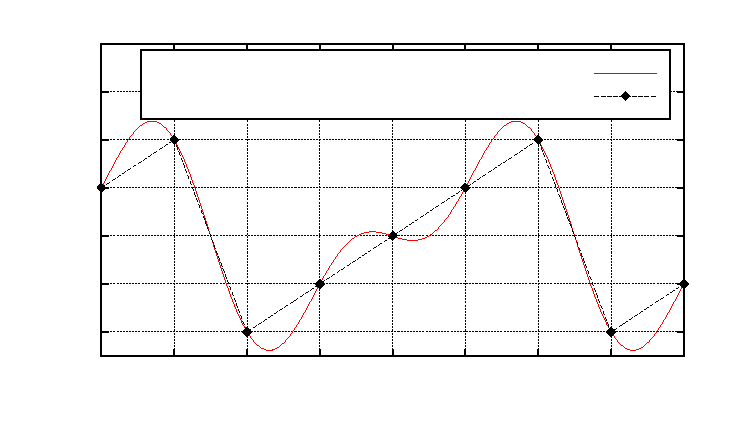
\includegraphics{example-1}}%
    \gplfronttext
  \end{picture}%
\endgroup

			\caption{trigonometrisches Polynom für Beispiel mit $n=4$ und der Funktion $\tilde{f}$}
			\label{fig:example}
		\end{figure}

		\textsc{Beispiel:}\\
		Sei nun $n=4$ und $\tilde{f}(k):=k$ für $k=0,1,2,3$. Dann lassen sich anhand der gegebenen Formeln die Fourier-Koeffizienten berechnen.
		Abbildung \ref{fig:example} zeigt das für diese Werte berechnete trigonometrische Interpolationspolynom.
		\begin{table}[h]
			\center
			\begin{tabular}{c|c|c|c}
				% \hline
				$\hat{f}(0)$ & $\hat{f}(1)$ & $\hat{f}(2)$ & $\hat{f}(3)$ \\
				\hline \hline
				$\dfrac{3}{2}$ & $-\dfrac{1}{2}+\dfrac{i}{2}$ & $-\dfrac{1}{2}$ & $-\dfrac{1}{2}-\dfrac{i}{2}$ \\
				% \hline
			\end{tabular}
			\caption{Fourierkoeffizienten für Beispiel mit $n=4$ und der Funktion $\tilde{f}$}
		\end{table}
		
	% subsection diskrete_fouriertransformation (end)

% section mathematische_grundlagen (end)

\section{Serieller Algorithmus} % (fold)
\label{sec:serieller_algorithmus}

	\subsection{Idee der Fast Fourier Transform} % (fold)
	\label{sub:idee_der_fast_fourier_transform}
	
		Eine naive Berechnung der diskreten Fouriertransformation nach obiger angegebener Formel führt pro Fourier-Koeffizient auf eine Anzahl von $n+1$ Multiplikationen und $n-1$ Additionen.
		Dabei wurde die Berechnung der Faktoren $e^{ix}$, die auch Twiddle-Faktoren genannt werden, außen vor gelassen.
		Diese können durch geeignete Tabellenwerte, die dem Programm vorab zur Verfügung gestellt werden, direkt abgelesen werden.
		Die Berechnung muss nun für alle $n$ Koeffizienten durchgeführt werden.
		Es ergeben sich damit also $n(n+1)$ Multiplikationen und $n(n-1)$ Additionen, welche für die Durchführung eines naiven Algorithmus benötigt werden würden.
		Bezeichnet nun mit $W(n)$ die Anzahl der Operation, die ein gegebener Algorithmus für $n$ Datenpunkte ausführt, dann folgt für einen naiven Algorithmus der diskreten Fouriertransformation
		\[ W(n) = \underbrace{n(n+1)}_{\mathclap{\mathrm{Multiplikation}}} + \underbrace{n(n-1)}_{\mathclap{\mathrm{Addition}}} = 2n^2 \in \Omega\curvb{n^2} \]
		Um dies zu verbessern, wird die Gleichung für die Fouriertransformation umgeformt, indem man zwischen geraden und ungeraden Summanden unterscheidet.
		Es sei nun $n=2m$ für ein $m\in\SN$ und $k\in\curlb{0,\ldots,n-1}$.
		\begin{alignat*}{3}
			\FF_n f(k) &=&& \ \frac{1}{n} \sum_{j=0}^{n-1} f(j)e^{-\frac{2\pi i}{n}kj} \\
			&=&& \ \frac{1}{n} \boxb{ \sum_{j=0}^{m-1} f(2j)e^{-\frac{2\pi i}{n}2kj} + \sum_{j=0}^{m-1} f(2j+1)e^{-\frac{2\pi i}{n}k(2j+1)} } \\
			&=&& \ \frac{1}{n} \sum_{j=0}^{m-1} f(2j)e^{-\frac{2\pi i}{n}2kj} + e^{-\frac{2\pi i}{n}k} \frac{1}{n} \sum_{j=0}^{m-1} f(2j+1)e^{-\frac{2\pi i}{n}2kj}
		\end{alignat*}
		Für $k<m$ können diese beiden Summen durch diskrete Fouriertransformationen für $m$ Punkte ersetzt werden.
		\begin{alignat*}{3}
			&\FF_n f(k) &&=&& \ \FF_m f(2\cdot)(k) + e^{-\frac{2\pi i}{n}k} \cdot\FF_m f(2\cdot+1)(k) \\
			\intertext{Um auch für andere Werte von $k$ die Gleichung zu bestimmen, addiert man $m$.}
			&\FF_n f(k+m) &&=&& \ \FF_m f(2\cdot)(k) - e^{-\frac{2\pi i}{n}k} \cdot\FF_m f(2\cdot+1)(k)
		\end{alignat*}
		Das Ausführen der Fouriertransformation für $n$ Punkte wird also auf die Ausführung zweier Fouriertransformationen für $n/2$ Punkte zurückgeführt.
		Man möchte nun durch ein rekursives Wiederholen dieser Prozedur die asymptotische Laufzeit verbessern.
		Aus diesem Grund wird nun $n=2^p$ für ein $p\in\SN$ gesetzt (es sind also $p$ rekursive Schritte möglich).
		Es ergibt sich dann folgendes Induktionsproblem für alle $k\in\curlb{1,\ldots,n/2}$:
		\begin{alignat*}{3}
			&W(2k) &&=&& \ 2W\curvb{k} + 4k \\
			&W(1) &&=&& \ 0 \\
			\\
			\Rightarrow \ &W(n) &&=&& \ 2np = 2n\log_2n \in \Omega(n\log_2n)
		\end{alignat*}
		Auch bei dieser Berechnung sind die Twiddle-Faktoren nicht mit einberechnet.
		Auf diese Art erfährt die Berechnung der diskreten Fouriertransformation eine signifikante Beschleunigung.
		Algorithmen der Fouriertransformation, die diese Zeitkomplexität aufweisen, werden im allgemeinen Fast Fourier Transform oder auch FFT genannt.

	% subsection idee_der_fast_fourier_transform (end)

	\subsection{Rekursiver Algorithmus} % (fold)
	\label{sub:rekursiver_algorithmus}
	
		Ein erster einfacher rekursiver FFT-Algorithmus ergibt sich nun direkt aus den oben definierten induktiven Gleichungen.


	% subsection rekursiver_algorithmus (end)

% section serieller_algorithmus (end)